%%%%
% Forcing line breaks in \url within bib latex
% https://tex.stackexchange.com/a/237684
%%%%
\PassOptionsToPackage{hyphens}{url}
%%%%
% LATEX Class for the Association for Computing Machinery
% https://www.acm.org/binaries/content/assets/publications/consolidated-tex-template/acmart.pdf
%%%%
\documentclass[sigplan, review]{acmart}

%%%%
% To use the SIGCHI extended abstract template, please visit
% https://www.overleaf.com/read/zzzfqvkmrfzn
%%%%

%%%%
% What packages do people load by default in LaTeX?
% https://tex.stackexchange.com/questions/553/what-packages-do-people-load-by-default-in-latex
%%%%
\usepackage{hyperref}
\usepackage{cleveref}
\usepackage{microtype} % refinements towards typographical
\usepackage{subcaption}
\usepackage{booktabs} % For formal tables
\usepackage{lipsum} % For placeholder text

%%%%
% CUSTOMISE ACMART DESIGN
% https://tex.stackexchange.com/a/346309
%%%%
\setcopyright{none}
\settopmatter{printacmref=false}
\renewcommand\footnotetextcopyrightpermission[1]{}
% \pagestyle{plain}

\acmConference[ACEAI]{Affective Computing / Empathic Artificial Intelligence}{2019-2020}{Munich, Germany}

\begin{document}

\title[BodyPose - Break Slouching Habits of the Digital Age]{BodyPose - Break Slouching Habits of the Digital Age:\\ Design and Evaluation of a Pose Monitoring Concept}

% AUTHOR
\author{Andreas Ellwanger}
\affiliation{%
  \institution{LMU Munich}
  \city{Munich}
  \state{Bavaria}
  \country{Germany}
}
\email{andreas.ellwanger@campus.lmu.de}
% AUTHOR
\author{Timo Erdelt}
\affiliation{%
  \institution{LMU Munich}
  \city{Munich}
  \state{Bavaria}
  \country{Germany}
}
\email{timo.erdelt@campus.lmu.de}
% AUTHOR
\author{Samantha Kühn}
\affiliation{%
  \institution{LMU Munich}
  \city{Munich}
  \state{Bavaria}
  \country{Germany}
}
\email{samantha.kuehn@campus.lmu.de}
% AUTHOR
\author{Johannes Tochtermann}
\affiliation{%
  \institution{LMU Munich}
  \city{Munich}
  \state{Bavaria}
  \country{Germany}
}
\email{johannes.tochtermann@campus.lmu.de}

%%%%
% ABSTRACT
%%%%
\begin{abstract}
\lipsum[2-3]
\end{abstract}

%%%%
% KEYWORDS
%%%%
\keywords{User interface, neural network.}

%%%%
% MAKE TITLE !!! DON'T MOVE
%%%%
\maketitle

%%%%
% IMPORT
%%%%
%%%
%%% Introduction
%%%
\section{Introduction} % in progress
\label{introduction}
% etliche Leute leiden eines Tages an Rückenschmerzen
% Besonders herausheben: Menschen, die an Rechnern arbeiten
% Problemfeld: degenerative Rückenerkrankungen durch zu lange falsche Haltung
% Unsere Lösung: BodyPose
% Unser Lösungsansatz: webapp die Haltungskorrekturen motiviert
% Unsere Lösung angwandt auf oben beschriebenes Problem
% In Richtung was es sonst noch so gibt -> Überleitung zu related works

Suffering from back pain is a severe but common constraint, that reduces everyday life quality. It tops the list of all reported work-related disorders~\cite{osha2000facts}. The outlook to this serious medical condition forecasts, that 60\% - 90\% of people will suffer from low back disorders at some point in their life~\cite{osha2000facts}. It is certain, that already 30\% of European workers suffer from back pain~\cite{osha2000facts}. As for 57 \% of all employees in EU the work environment includes working on laptops/computers on a daily basis (2019)~\cite{eurostat_comp_use}, it is necessary that precaution tools as well as education are provided for employees in order to prevent them from getting back pain. The European Agency for Safety and Health at work states, that "exposure to ergonomic risks factors represents one of the major occupational safety and health problems in the EU today. Repeated exposure to these risks can result in work-related musculoskeletal disorders — one of the most serious and widespread work-related illnesses, which give rise to major cost burden for individuals, businesses and society in general."~\cite{osha2019msd}

Motivated from this severe long term health threat starting point, we designed the web app BodyPose. While running in background, it encourages users to maintain or realign their posture. BodyPose observes the user's posture via webcam, which is then recognised by the underlying PoseNet model. The out coming data points are evaluated by a rule-based system, which triggers notifications to the user in case of misalignment. Users can adjust the sensitivity of the notification threshold to their liking for different body parts independently. BodyPose is designed as light-weight application, which can be run on various devices supporting web browser, to allow users to stay flexible within their preferred working devices.

%Brauchbarer Übergang zu related works?

%%%
%%% Related Work
%%%
\section{Related Work} % in progress
\label{related-work}
The idea of designing a system that can monitor and evaluate the upper body posture of a user is not novel. However, most of the previous work, such as ~\cite{demmans2007posture}, requires the use of sensors. This is also the case with the \textit{Upright Go} product line~\footnote{\href{https://www.uprightpose.com/}}, a solution that is already on the market. In contrast to this, our application only requires input from a webcam. Jaimes et al.~\cite{jaimes2005sit} also use camera input. 

To our knowledge, the only approach using camera input is ~\cite{jaimes2005sit}. In contrast to ~\cite{jaimes2005sit}, however, BodyPose requires only camera input
% Ähnliche Produkte

% Gleiches Konzept, aber ausschließlich regelbasiert

%"Posture monitoring and improvement for laptop use."~\cite{demmans2007posture}

%“Sit straight (and tell me what I did today): a human posture alarm and activity summarization system”~\cite{jaimes2005sit}

\section{Technology} % in progress
\subsection{Components} % in progress
\begin{itemize}
    \item PoseNet model
    \item rule-based system
    \item feedback system
    \item statistics
\end{itemize}

%\section{Medical consultation} % in progress

%%%
%%% User Study 1
%%%
\section{User Study} % in progress
\label{user-study-1}
We designed a user study in which we examined the effects of BodyPose on postural habits. Particularly, we were interested in measuring the user experience of BodyPose as well as the short and long term motivation on correcting unhealthy postural misalignment due to the usage of BodyPose. As it is intended for operating while working on Laptops and PCs, we focused the study setup on workplace environment.

\subsection{Study Design}
\label{us1-study-design}
As the study was intended to be a test study, we implemented it as a laboratory study. Therefore we controlled potential confounding variables such as workplace lightning, hardware and network stability.
The study focuses on gaining insight regarding user experience and motivational effects of BodyPose on maintaining or realigning to a healthy posture.\\
Evaluating web-based user interfaces is not trivial, but has been carried out before. Researchers have used different metrics to identify various relevant aspects in the past. These can be (among others) the workload that a system provokes~\cite{hart1988development,hart2006nasa}, the creativity support that it provides~\cite{cherry2014quantifying}, the sense of control a user perceives~\cite{dong2015development}.

% It should be noted, however, that this study is considered to be a test run. To gain reliable results and insights, a higher number of participants, as well as a more controlled and isolated setup are required.

\subsection{Measurements}
\label{us1-measurements}
In order to measure the user experience and motivational effects, we used two surveys.\\
Firstly, we designed a survey to gather quantitative personal information as body height and weight as well as qualitative information referring to the participant's back pain history. These information will be used to classify how severe the participants' back pain condition already is. Additionally we asked about various user interface impressions and motivational impact of BodyPose in short and long term. These questions were to be answered on a 5-point-scale.\\
Furthermore, we utilised an extended version of the NASA-TLX~\cite{hart2006nasa} to collect quantified data at the end of the task. The questionnaire measured workload, sense of control and creativity support. The Task-Load Index (TLX) from NASA~\cite{hart2006nasa} measured the subjective amount of workload experienced by the participants. The sense of control scale by Dong et al.~\cite{dong2015development} adapted to a 20-point rating scale measured perceived control. Lastly, Creativity Support Index by Cherry et al.~\cite{cherry2014quantifying}, limited to exploration, motivation and enjoyment dimensions measured the creativity support.

\subsection{Study Tasks}
\label{us1-tasks}
We defined three phases within the user study. Phase one gives the participants an overview of the features of BodyPose and encourages to explore them on their own. As BodyPose is designed for background usage, phase two simulates an every day's work task. Lastly, the participants are invited to fill in a survey consisting of the in \ref{us1-measurements} described questionnaires.

\begin{description}
\item[In-App task:]  Overview of features\\
Please follow the given instructions while BodyPose is activated. 
\begin{itemize}
	\item Activate camera feed
	\item Deactivate and reactivate browser notifications
	\item Go to settings and experiment with them by adjusting the threshold parameters: Observe the effect on the App's functionalities caused by these changes.
\end{itemize}

\item[Out-of-App task:]  Simulation of a work task
\begin{itemize}
	\item Write down your favourite recipe and add a representative picture (from the internet) to your text
\end{itemize}

\item[Questionnaires] on the study task
\begin{itemize}
	\item Survey on
	\begin{itemize}
		\item Personal questions regarding back health history
	    \item Questions regarding the app's usability
		\item Questions regarding motivational effects of BodyPose
	\end{itemize}
	\item Extended NASA TLX survey on evaluating the subjective perception of the task's
	\begin{itemize}
		\item Workload
		\item Sense of control
		\item Creativity support
	\end{itemize}
\end{itemize}
\end{description}


\subsection{Procedure}
\label{us1-procedure}
In beforehand we prepared three of our already tested devices by launching a browser with BodyPose and both questionnaires.
The participants were instructed to use BodyPose according to the in \ref{us1-tasks} described tasks and fill in the given surveys. There were no time constraints given as well as no signal to when to proceed to the next task, as we wanted to keep the focus of the participants on exploring BodyPose freely.
  

\subsection{Participants}
\label{us1-participants}
In this test study, our fellow computer sciences colleagues participated. Two of them were male, one female and their average age was 24, ranging from 23 to 27.


\subsection{Data Analysis and Results}
\label{us1-data-analysis-results}
Evaluating both questionnaires described in \ref{us1-measurements}, we gathered various insights.
Firstly, it can be seen in \ref{fig:us-gs-shortterm}, that all participants felt motivated to correct their body posture immediately when BodyPose notified them having slouched into an unhealthy alignment.
Furthermore, as the chart in \ref{fig:us-gs-longterm} depicts, all participants stated, that BodyPose encourages them to increase their emphasis on being aware of their body posture.
And lastly, the results of the extended NASA TLX questionnaire, as shown in \ref{fig:ext-nasa-results}, state, that the participants rated the workload intensity at 43\% with a standard deviation of 5,4\%. Furthermore they felt in sense of control during the task to 62\% with a with a standard deviation of 13\%. Lastly, they classified their subjective perception of creativity support at 71\% with a standard deviation of 12\%.

\begin{figure}[hbp]
\centering
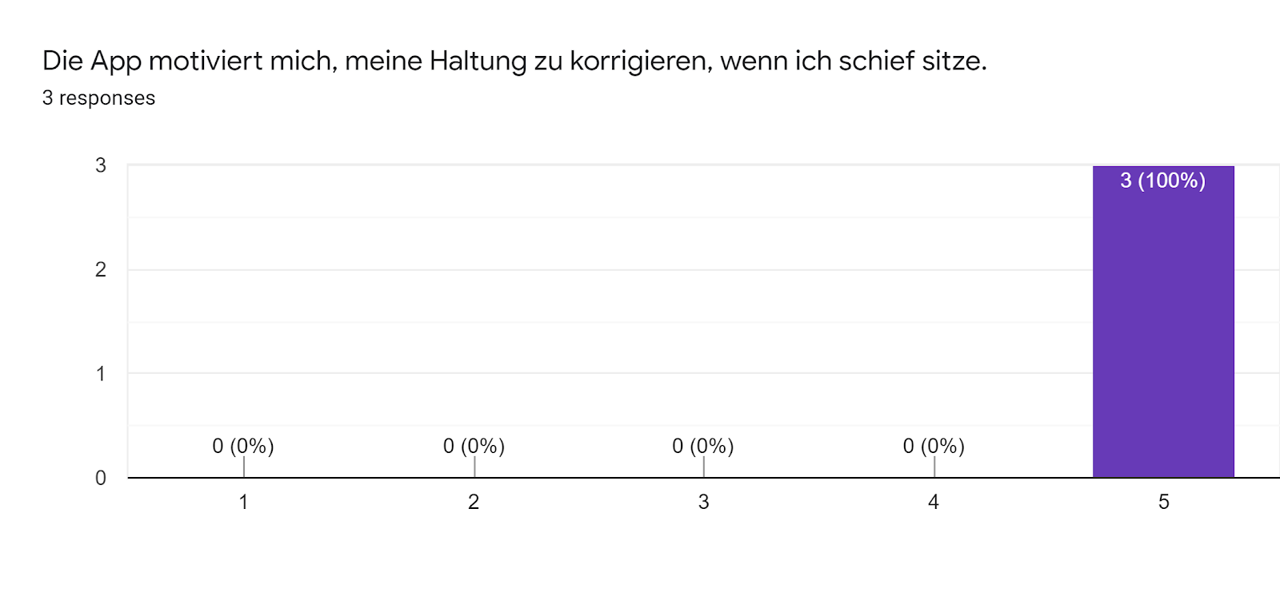
\includegraphics[width=\linewidth]{media/us-gs-shortterm-motivation-results.png}    
\caption{Short-term motivation}
\label{fig:us-gs-shortterm}
\end{figure}

\begin{figure}[hbp]
\centering
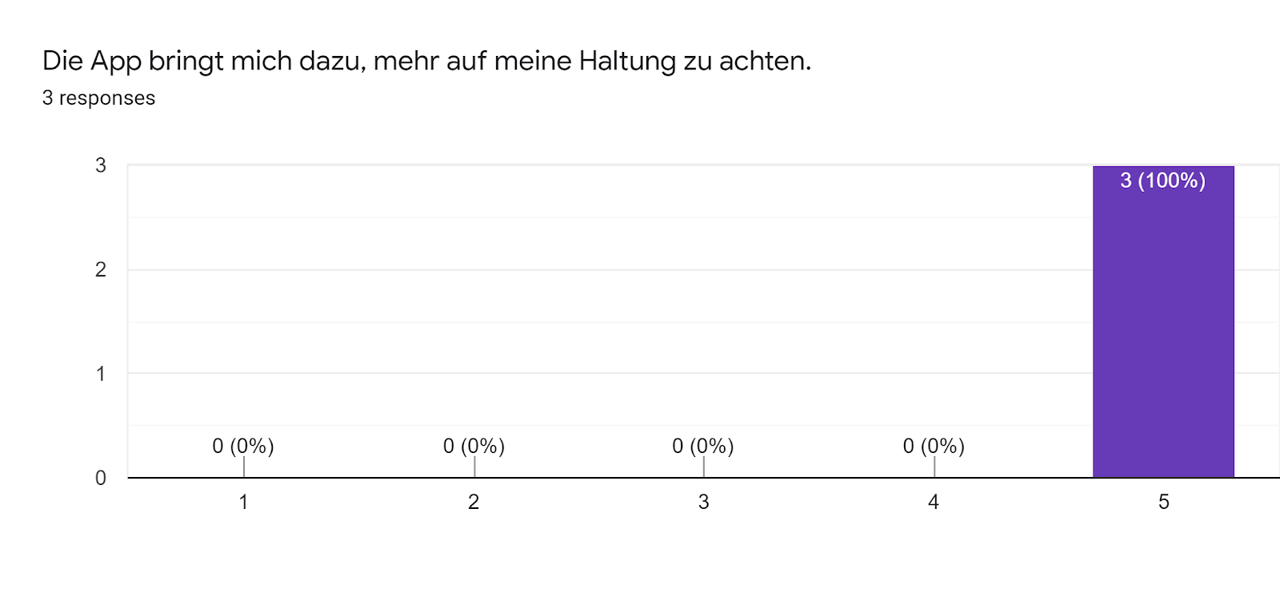
\includegraphics[width=\linewidth]{media/us-gs-longterm-motivation-results.png}    
\caption{Long-term motivation}
\label{fig:us-gs-longterm}
\end{figure}

\begin{figure}[hbp]
\centering
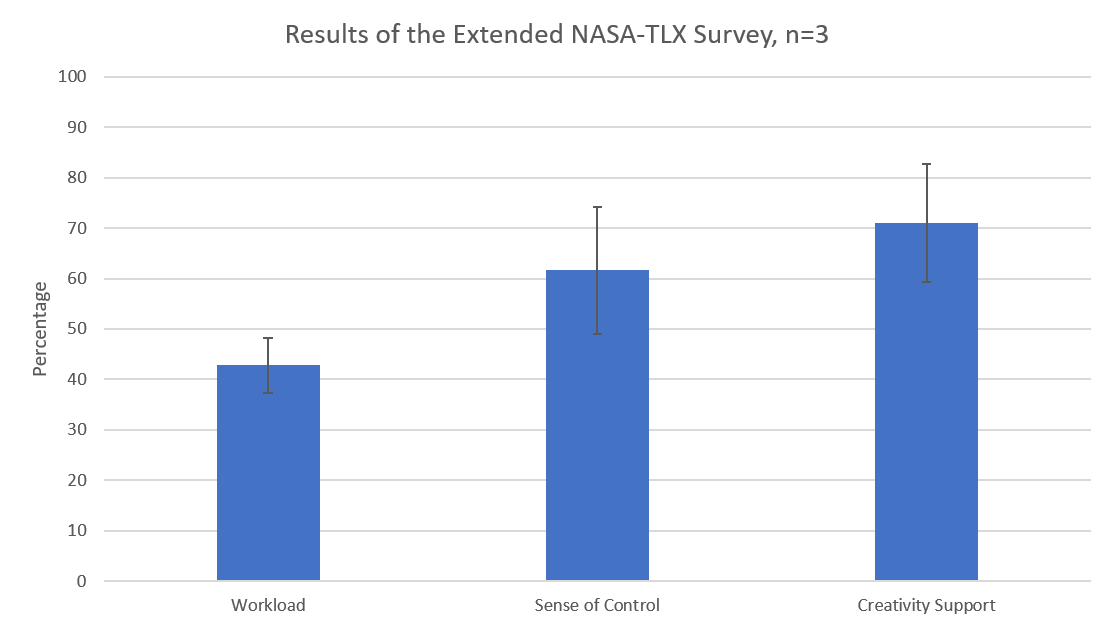
\includegraphics[width=\linewidth]{media/us-ext-nasa-tlx-results.png}    
\caption{Bar charts regarding workload, sense of control and creativity support}
    \label{fig:ext-nasa-results}
\end{figure}

%%%
%%% Discussion and future work
%%%
\section{Discussion} % in progress
\label{discussion-future-work}


\subsection{User Study Procedure}
As only three participants took part in our user study, the results shown in \ref{us1-data-analysis-results} are statistically not representative. Furthermore, execution of the user study did not strictly follow the study protocol described in \ref{us1-procedure}: Since our participants were aware they were being observed not only by us but also by our mentors and colleagues, their behaviour might also not have been representative. Additionally, participants were not isolated from each other, so they did not perform their tasks independently. Lastly, since we recruited the participants from amongst our co-students, it can not be ruled out that personal bias(es) might have influenced the result.


%%%
%%% Conclusion
%%%
\section{Conclusion} % in progress
\label{conclusion}

% \lipsum[2-4]
\section{Future Work}
\begin{itemize}
    \item let model learn rule-based system
\end{itemize}
There are several potential future avenues worth pursuing in order to enhance and improve the functionality of BodyPose: To allow for a more personalised user experience, users should be able to create an account and save not only their settings (such as threshold values) but also calibration and session data (such as statistics). Furthermore, implementing a user identification system via face detection might prove helpful for robustness: since BodyPose uses PoseNet's single-pose detection algorithm, the system can not handle situations robustly where multiple persons are visible to the camera. Identifying users with face detection could mitigate this problem, as the system could be modified only to evaluate the pose of persons who can be identified as the currently logged in user. Another avenue for improving robustness, as well as accuracy, lies in replacing the pose detection model itself: PoseNet detects poses in two dimensions, but some models can detect poses in three dimensions, even from two-dimensional input, such as in \cite{Arnab_2019}. This model shows improved robustness and accuracy when compared to two-dimensional pose detection. However, due to the added complexity, this could potentially result in a trade-off regarding performance.

\appendix
%Appendix A
%\section{User Study 1: Visual search task}

%\begin{figure}[hbp]
%\centering
%\includegraphics[width=\linewidth]{media/us1.png}    
%\caption{Layer setup}
%\label{fig:us1layers}
%\end{figure}

\begin{acks} % in progress
  The authors would like to thank all three participants for their participation in the user study, as well as Dr. Marco Meier, HYVE and TAWNY staff for their mentoring.
\end{acks}

%%%%
% BIBLIOGRAPHY
%%%%
\bibliographystyle{ACM-Reference-Format}
\bibliography{bibliography}

\end{document}
